\documentclass[futureinternet,article,submit,moreauthors,pdftex,10pt,a4paper]{Definitions/mdpi} 
\usepackage{algorithm}
\usepackage{algorithmicx}
\usepackage{amsmath}
\usepackage{algpseudocode}
\renewcommand{\algorithmicrequire}{\textbf{Input:}}  % Use Input in the format of Algorithm
\renewcommand{\algorithmicensure}{\textbf{Output:}} % Use Output in the format of Algorithm
\usepackage{amsthm}
\usepackage{amsmath}
\usepackage{enumitem}
\usepackage{graphicx}
\usepackage{subfigure}
\usepackage{color} %red, green, blue, yellow, cyan, magenta, black, white
\definecolor{mygreen}{RGB}{28,172,0} % color values Red, Green, Blue
\definecolor{mylilas}{RGB}{170,55,241}
\newlist{steps}{enumerate}{1}
\setlist[steps, 1]{label = Step \arabic*).}
\theoremstyle{plain}
\newtheorem{thm}{Theorem}[section]
\newtheorem{lem}[thm]{Lemma}
\newtheorem{prop}[thm]{Proposition}
\newtheorem*{cor}{Corollary}

\theoremstyle{definition}
\newtheorem{defn}{Definition}[section]
\newtheorem{conj}{Conjecture}[section]
\newtheorem{exmp}{Example}[section]

\theoremstyle{remark}
\newtheorem*{rem}{Remark}
\newtheorem*{note}{Note}
% If you would like to post an early version of this manuscript as a preprint, you may use preprint as the journal and change 'submit' to 'accept'. The document class line would be, e.g., \documentclass[preprints,article,accept,moreauthors,pdftex,10pt,a4paper]{mdpi}. This is especially recommended for submission to arXiv, where line numbers should be removed before posting. For preprints.org, the editorial staff will make this change immediately prior to posting.

%
%--------------------
% Class Options:
%--------------------
% journal
%----------
% Choose between the following MDPI journals:
% acoustics, actuators, addictions, admsci, aerospace, agriculture, agronomy, algorithms, animals, antibiotics, antibodies, antioxidants, applsci, arts, asi, atmosphere, atoms, axioms, batteries, bdcc, behavsci, beverages, bioengineering, biology, biomedicines, biomimetics, biomolecules, biosensors, brainsci, buildings, carbon, cancers, catalysts, cells, ceramics, challenges, chemengineering, chemosensors, children, cleantechnol, climate, clockssleep, cmd, coatings, colloids, computation, computers, condensedmatter, cosmetics, cryptography, crystals, cybersecurity, data, dentistry, designs, diagnostics, dairy, diseases, diversity, drones, econometrics, economies, education, electrochem, electrochemistry, electronics, energies, entropy, environments, epigenomes, est, fermentation, fibers, fire, fishes, fluids, foods, forecasting, forests, fractalfract, futureinternet, galaxies, games, gastrointestdisord, gels, genealogy, genes, geohazards, geosciences, geriatrics, hazardousmatters, healthcare, heritage, highthroughput, horticulturae, humanities, hydrology, informatics, information, infrastructures, inorganics, insects, instruments, ijerph, ijfs, ijms, ijgi, ijtpp, inventions, j, jcdd, jcm, jcs, jdb, jfb, jfmk, jimaging, jof, jintelligence, jlpea, jmmp, jmse, jpm, jrfm, jsan, land, languages, laws, life, literature, logistics, lubricants, machines, magnetochemistry, make, marinedrugs, materials, mathematics, mca, medsci, medicina, medicines, membranes, metabolites, metals, microarrays, micromachines, microorganisms, minerals, modelling, molbank, molecules, mps, mti, nanomaterials, ncrna, neonatalscreening, neuroglia, nitrogen, nutrients, ohbm, particles, pathogens, pharmaceuticals, pharmaceutics, pharmacy, philosophies, photonics, plants, plasma, polymers, polysaccharides, proceedings, processes, proteomes, publications, quaternary, qubs, reactions, recycling, religions, remotesensing, reports, resources, risks, robotics, safety, sci, scipharm, sensors, separations, sexes, sinusitis, smartcities, socsci, societies, soilsystems, sports, standards, stats, surfaces, surgeries, sustainability, symmetry, systems, technologies, toxics, toxins, tropicalmed, universe, urbansci, vaccines, vehicles, vetsci, vibration, viruses, vision, water, wem, wevj
%---------
% article
%---------
% The default type of manuscript is article, but can be replaced by: 
% abstract, addendum, article, benchmark, book, bookreview, briefreport, casereport, changes, comment, commentary, communication, conceptpaper, correction, conferenceproceedings, conferencereport, expressionofconcern, extendedabstract, meetingreport, creative, datadescriptor, discussion, editorial, essay, erratum, hypothesis, interestingimages, letter, meetingreport, newbookreceived, opinion, obituary, projectreport, reply, reprint, retraction, review, perspective, protocol, shortnote, supfile, technicalnote, viewpoint
% supfile = supplementary materials
% protocol: If you are preparing a "Protocol" paper, please refer to http://www.mdpi.com/journal/mps/instructions for details on its expected structure and content.
%----------
% submit
%----------
% The class option "submit" will be changed to "accept" by the Editorial Office when the paper is accepted. This will only make changes to the frontpage (e.g., the logo of the journal will get visible), the headings, and the copyright information. Also, line numbering will be removed. Journal info and pagination for accepted papers will also be assigned by the Editorial Office.
%------------------
% moreauthors
%------------------
% If there is only one author the class option oneauthor should be used. Otherwise use the class option moreauthors.
%---------
% pdftex
%---------
% The option pdftex is for use with pdfLaTeX. If eps figures are used, remove the option pdftex and use LaTeX and dvi2pdf.

%=================================================================
\firstpage{1} 
\makeatletter 
\setcounter{page}{\@firstpage} 
\makeatother
\pubvolume{xx}
\issuenum{1}
\articlenumber{5}
\pubyear{2018}
\copyrightyear{2018}
%\externaleditor{Academic Editor: name}
\history{Received: date; Accepted: date; Published: date}
%\updates{yes} % If there is an update available, un-comment this line

%% MDPI internal command: uncomment if new journal that already uses continuous page numbers 
%\continuouspages{yes}

%------------------------------------------------------------------
% The following line should be uncommented if the LaTeX file is uploaded to arXiv.org
%\pdfoutput=1

%=================================================================
% Add packages and commands here. The following packages are loaded in our class file: fontenc, calc, indentfirst, fancyhdr, graphicx, lastpage, ifthen, lineno, float, amsmath, setspace, enumitem, mathpazo, booktabs, titlesec, etoolbox, amsthm, hyphenat, natbib, hyperref, footmisc, geometry, caption, url, mdframed, tabto, soul, multirow, microtype, tikz

%=================================================================
%% Please use the following mathematics environments: Theorem, Lemma, Corollary, Proposition, Characterization, Property, Problem, Example, ExamplesandDefinitions, Hypothesis, Remark, Definition
%% For proofs, please use the proof environment (the amsthm package is loaded by the MDPI class).

%=================================================================
% Full title of the paper (Capitalized)
\Title{Efficient Tensor Sensing For RF Tomographic Imaging on GPUs}

% Author Orchid ID: enter ID or remove command
%\newcommand{\orcidauthorA}{0000-0000-000-000X} % Add \orcidA{} behind the author's name
%\newcommand{\orcidauthorB}{0000-0000-000-000X} % Add \orcidB{} behind the author's name

% Authors, for the paper (add full first names)
\Author{Da Xu $^{1}$ and Tao Zhang $^{1,2}$*}

% Authors, for metadata in PDF
\AuthorNames{Da Xu and Tao Zhang}

% Affiliations / Addresses (Add [1] after \address if there is only one affiliation.)
\address{%
$^{1}$ \quad Department of Computer Engineering and Science, Shanghai University, Shanghai,  China 200444; mr\_tab@shu.edu.cn\\
$^{2}$ \quad Shanghai Institute for Advanced Communication and Data Science, Shanghai, China; }

% Contact information of the corresponding author
\corres{Correspondence: taozhang@shu.edu.cn; Tel.: +86-21-66135300}

% Current address and/or shared authorship
%\firstnote{Current address: Affiliation 3} 
%\secondnote{These authors contributed equally to this work.}
% The commands \thirdnote{} till \eighthnote{} are available for further notes

%\simplesumm{} % Simple summary

%\conference{} % An extended version of a conference paper

% Abstract (Do not insert blank lines, i.e. \\) 
\abstract{Radio-frequency (RF) tomographic imaging is a promising technique for inferring multi-dimensional physical space by processing RF signals traversed across a region of interest. Tensor based approaches for tomographic imaging are superior in detecting the objects within higher dimensional spaces. The recently proposed tensor sensing approach based on the transform tensor model achieves lower error rate and faster speed than previous tensor-based compress sensing approach. However, the running time of the tensor sensing approach increases exponentially with the dimension of tensors, thus not very practical for big tensors. In this paper, we address this problem by exploiting massively parallel GPUs. We design, implement and optimize the tensor sensing approach on an NVIDIA Tesla GPU  and evaluate the performance in terms of the running time and recovery error rate. Experiment results show that our GPU tensor sensing is as accurate as the CPU counterpart with an average of $44.79 \times$ and up to $84.70 \times$ speedups for varying sized synthetic tensor data. For ground-truth 3D model data of smaller size, our GPU algorithm achieves 15.37x speedup over the CPU tensor sensing. We further encapsulate the GPU algorithm into an open-source library, called \textit{cuTensorSensing}, which can be used for efficient RF tomographic imaging.}

% Keywords
\keyword{Radio frequency; tomographic imaging; tensor; GPU}

% The fields PACS, MSC, and JEL may be left empty or commented out if not applicable
%\PACS{J0101}
%\MSC{}
%\JEL{}

%%%%%%%%%%%%%%%%%%%%%%%%%%%%%%%%%%%%%%%%%%
% Only for the journal Diversity
%\LSID{\url{http://}}

%%%%%%%%%%%%%%%%%%%%%%%%%%%%%%%%%%%%%%%%%%
% Only for the journal Applied Sciences:
%\featuredapplication{Authors are encouraged to provide a concise description of the specific application or a potential application of the work. This section is not mandatory.}
%%%%%%%%%%%%%%%%%%%%%%%%%%%%%%%%%%%%%%%%%%

%%%%%%%%%%%%%%%%%%%%%%%%%%%%%%%%%%%%%%%%%%
% Only for the journal Data:
%\dataset{DOI number or link to the deposited data set in cases where the data set is published or set to be published separately. If the data set is submitted and will be published as a supplement to this paper in the journal Data, this field will be filled by the editors of the journal. In this case, please make sure to submit the data set as a supplement when entering your manuscript into our manuscript editorial system.}

%\datasetlicense{license under which the data set is made available (CC0, CC-BY, CC-BY-SA, CC-BY-NC, etc.)}

%%%%%%%%%%%%%%%%%%%%%%%%%%%%%%%%%%%%%%%%%%
% Only for the journal Toxins
%\keycontribution{The breakthroughs or highlights of the manuscript. Authors can write one or two sentences to describe the most important part of the paper.}

%\setcounter{secnumdepth}{4}
%%%%%%%%%%%%%%%%%%%%%%%%%%%%%%%%%%%%%%%%%%
\begin{document}
%%%%%%%%%%%%%%%%%%%%%%%%%%%%%%%%%%%%%%%%%%
%% Only for the journal Gels: Please place the Experimental Section after the Conclusions

%%%%%%%%%%%%%%%%%%%%%%%%%%%%%%%%%%%%%%%%%%
%\setcounter{section}{-1} %% Remove this when starting to work on the template.
%\section{How to Use this Template}
%The template details the sections that can be used in a manuscript. Note that the order and names of article sections may differ from the requirements of the journal (e.g., the positioning of the Materials and Methods section). Please check the instructions for authors page of the journal to verify the correct order and names. For any questions, please contact the editorial office of the journal or support@mdpi.com. For LaTeX related questions please contact Janine Daum at latex-support@mdpi.com.
%The order of the section titles is: Introduction, Materials and Methods, Results, Discussion, Conclusions for these journals: aerospace,algorithms,antibodies,antioxidants,atmosphere,axioms,biomedicines,carbon,crystals,designs,diagnostics,environments,fermentation,fluids,forests,fractalfract,informatics,information,inventions,jfmk,jrfm,lubricants,neonatalscreening,neuroglia,particles,pharmaceutics,polymers,processes,technologies,viruses,vision

\section{Introduction}
\begin{figure}[H]
\centering
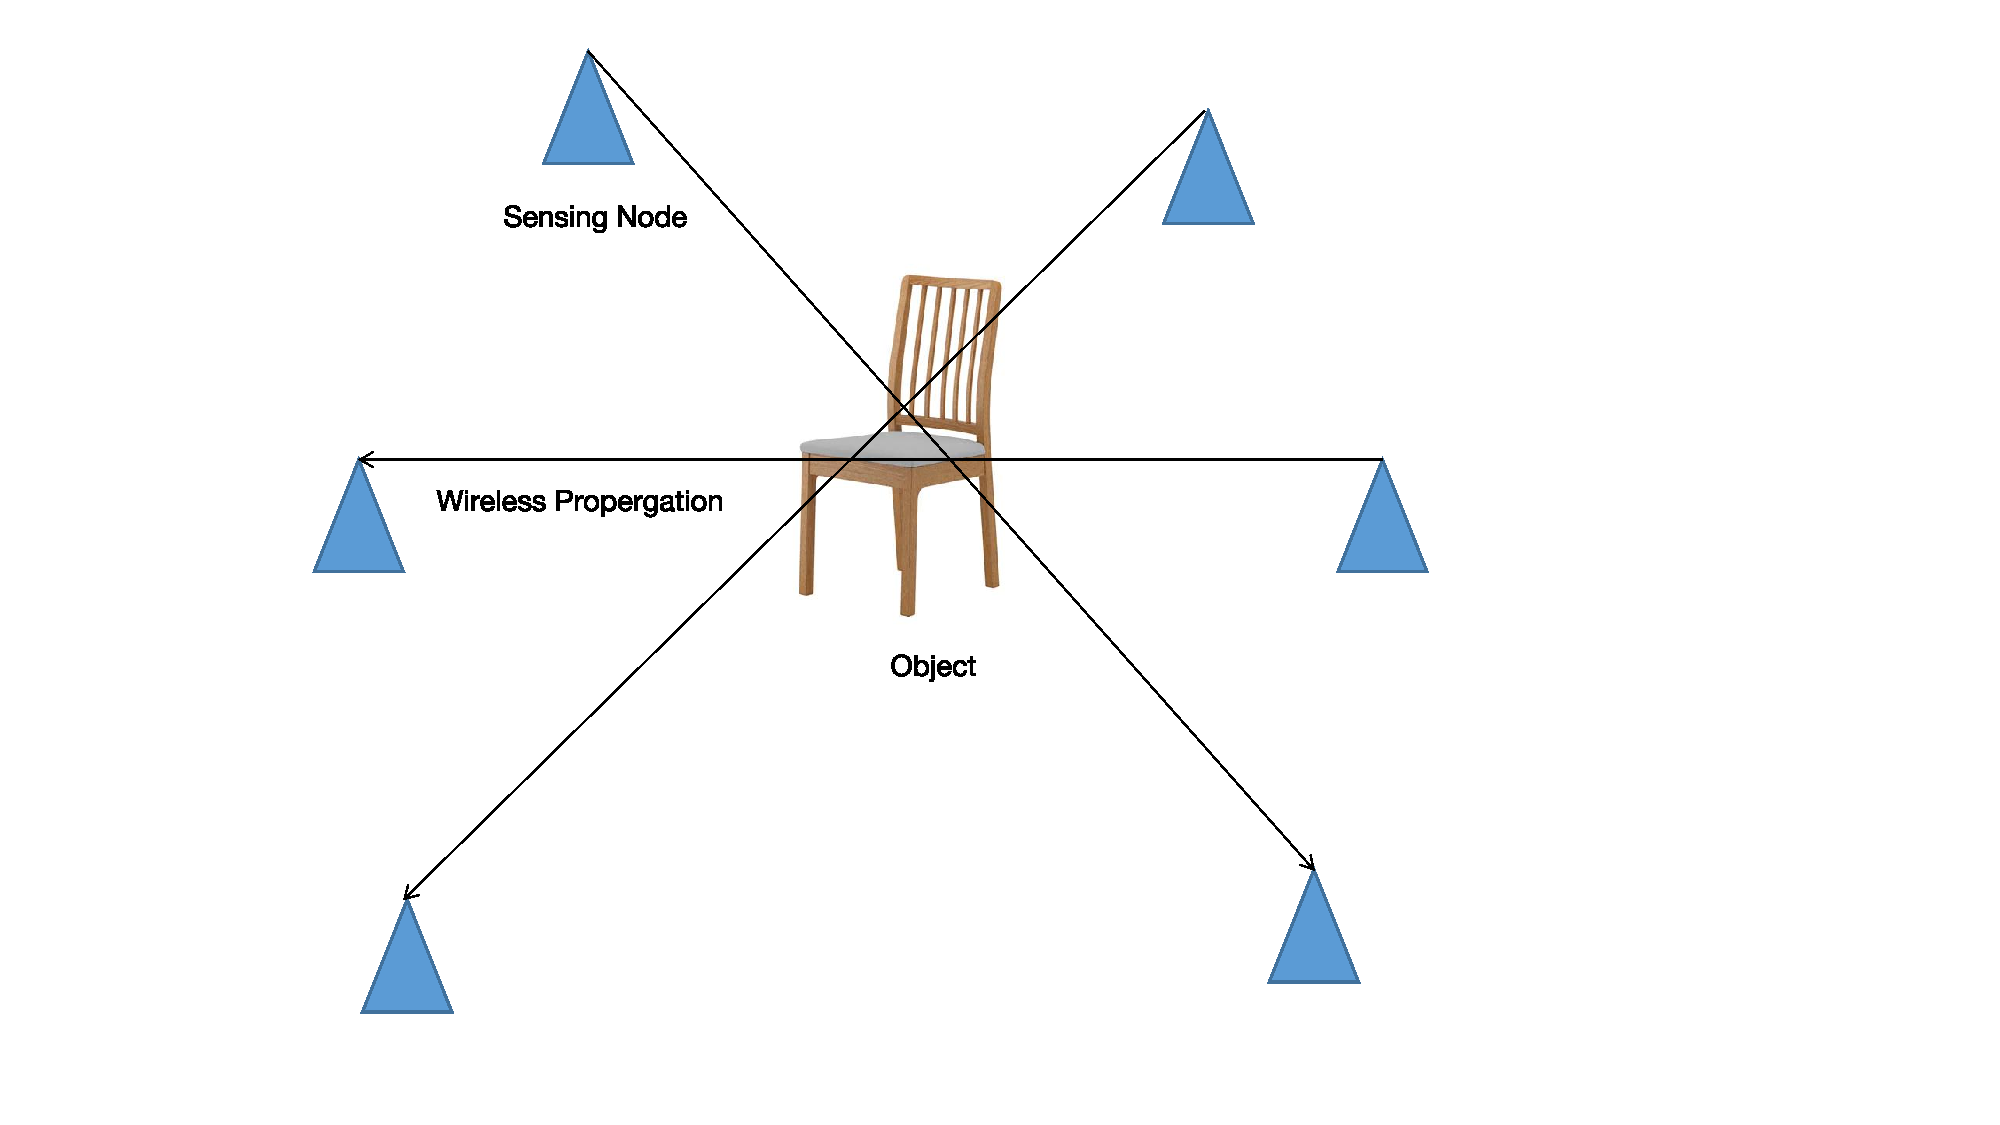
\includegraphics[width=0.7\textwidth]{RF.pdf}
\caption{An illustration of RF tomographic imaging network}
\label{Fig:RF}
\end{figure}
Radio frequency (RF) tomographic imaging, also called wireless tomography, is a technique for detecting objects within a specific region by analyzing radio frequency signals transmitted between wireless nodes, as shown in Fig. \ref{Fig:RF}. This technique uses radio reflections that bounce off the object body and does not require the object to carry any wireless device. This advantage has made it ideal for security checking, rescue operations, space applications, and smart buildings \cite{matsuda2017multi}.

In general, wireless signal propagating on a link loses power due to shadowing, distance and multipath fading. The task of RF tomographic imaging is to estimate a spatial distribution of the shadowing loss in a detecting region from measured power of wireless signals. A tensor-based compressed sensing method \cite{matsuda2017multi} was proposed for RF tomographic imaging in a three and higher dimensionally structured region, which estimates the distribution by utilizing its low-rank property. However, the method requires computing tensor singular value decomposition (t-SVD) in each algorithmic iteration, which leads to high computational complexity. To address this problem, Deng et al. \cite{deng2018tensor} proposed to use the transform-based tensor model to formulate the RF tomographic imaging as a tensor sensing problem, then use a fast iterative algorithm Alt-Min to solve the tensor sensing problem. Their method fully utilizes the geometric structure of the three-dimensional loss field tensor. Compared to the tensor-based compressed sensing method, Deng's method achieved lower error rate and faster computation speed.

However, the iterative algorithm Alt-Min proposed by Deng et al.\cite{deng2018tensor} iteratively estimates a pair of tensors, which is a computationally-intensive process, thus not very practical for RF tomographic imaging for big objects or regions, or real-time applications. In this paper, we address this problem by exploiting Graphics Processing Units (GPUs). Because of massive hardware parallelism and high memory bandwidth, GPUs have been widely used in diverse applications including machine learning \cite{cui2016geeps} \cite{brito2017detecting} \cite{campos2017scaling}, graph processing \cite{shi2018frog} \cite{zhong2017optimizing} \cite{pan2017multi}, big data analytic \cite{gutierrez2017smote} \cite{rathore2017real}, image processing \cite{devadithya2017gpu}, and fluid dynamics \cite{verma2017advanced}. In order to reap the power of GPUs, the algorithmic steps need to be mapped delicately onto the architecture of GPUs, especially the thread and memory hierarchy.  In this work, we design, implement and optimize the transform model based tensor sensing method of Deng et al. \cite{deng2018tensor} on an NVIDIA Tesla V100 GPU with CUDA (Compute Unified Device Architecture) and evaluate it in terms of the running time and recovery error. Experiment results show that the GPU algorithm achieves similar relative error as the CPU counterpart. Moreover, the GPU tensor sensing outperforms the CPU tensor sensing on all tensor sizes with 45.39x speedup on average and up to 84.70x speedup on bigger tensor size such as $120 \times 120 \times 6$. We encapsulate this GPU tensor sensing algorithm into an open-source library called ``cuTensorSensing" (CUDA Tensor Sensing) which is available at: http://www.findai.net.

Our contributions are summarized as follows. First, we analyze the steps of transform model based tensor sensing using the Alt-Min algorithm and discuss how to map them onto the GPU architecture. Second, we design, implement and optimize the tensor sensing on an NVIDIA Tesla V100 GPU. Third, we evaluate and compare the GPU tensor sensing and the CPU tensor sensing in terms of running time and relative error with both synthetic data and ground-truth data. Fourth, we encapsulate the GPU tensor sensing implementation into an open-source library such that it can be used in diverse applications.

The remainder of the paper is organized as follows. In Section \ref{SEC_RW}, we discuss the related works. Section \ref{SEC_ALGORITHM} presents the notations and briefly summarizes the RF tomographic imaging task as a tensor sensing problem. Section \ref{SEC_GPU} describes the design, implementation and optimizations of the tensor sensing on the GPU. In Section \ref{SEC_EXP}, we describe the experiment methology. Section \ref{SEC_RESULT} evaluates the GPU tensor sensing with both synthetic data and ground-truth data. The conclusions are given in Section \ref{SEC_CON}.

\section{Related Works}
\label{SEC_RW}
Existing works on RF tomographic imaging can be classified into vector-based and tensor-based approaches. The vector-based approaches \cite{kanso2009compressed} \cite{mostofi2011compressive} aim at estimating a spatial distribution of the shadowing loss in 2D regions of interest. They are not able to infer three-dimensional regions due to the fact that spatial structures of the signal data are ignored. Therefore, researchers have proposed the tensor-based approaches \cite{matsuda2017multi} \cite{deng2018tensor} to infer higher dimensional spaces of 3D and above. The tensor-based compressed sensing \cite{matsuda2017multi} used tensor nuclear norm (TNN) \cite{li2013generalized} to extend RF tomographic problems to three-dimensional case. This approach has high computational complexity and error rate. Deng et al. \cite{deng2018tensor} exploited the transform-based tensor model \cite{liu2017fourth} to explore three-dimensional spatial structures for higher accuracy and speed. Our work aims at accelerate Deng's work on GPUs to make it practical for real-time scenarios and bigger tensors.

GPUs have massive parallelism and high memory bandwidth, and many existing researches \cite{jing2016energy} \cite{zhang2015buddy} \cite{zhang2015efficient} \cite{zhang2014cuirre} \cite{zhang2016efficient} have demonstrated the benefit of utilizing GPUs to accelerate general purpose computing. Due to the high dimensions of tensors, tensor computations are often computation-intensive and time consuming. Recently, GPUs have been increasingly adopted to accelerate diverse tensor computations. Some works focus on accelerating specific tensor operations including tensor contraction \cite{nelson2015generating} \cite{shi2016tensor}, factorization \cite{antikainen2011nonnegative}, transpose \cite{lyakh2015an} \cite{hynninen2017cutt}, and tensor-matrix multiplication \cite{rogers2016efficient}. These works propose parallel tensor algorithms specifically optimized for the GPU architectures. GPUTENSOR \cite{zou2015gputensor} is a parallel tensor factorization algorithm that splits a tensor into smaller blocks and exploits the inherent parallelism and high-memory bandwidth of GPUs. To handle dynamic tensor data, GPUTENSOR updates its previously factorized components instead of recomputing them from the raw data. Sparse tensor-times-dense matrix multiply is a critical bottleneck in data analysis and mining applications and \cite{li2016optimizing} proposed an efficient primitive on CPU and GPU platforms. Different with these works, our work considers the tensor sensing based on the transform tensor model for RF tomographic imaging.

%%%%%%%%%%%%%%%%%%%%%%%%%%%%%%%%%%%%%%%%%%
\section{Description of the Tensor Sensing Problem}
\label{SEC_ALGORITHM}
Deng et al. \cite{deng2018tensor} proposed to use the transform-based tensor model to formulate the RF tomographic imaging as a tensor sensing problem. Then they utilized a fast iterative algorithm Alt-Min to solve the tensor sensing problem. Here we briefly summarize their approach including the Alt-Min algorithm in order to map it onto the GPU architecture.

\subsection{Alt-Min Algorithm}
    The goal of tensor sensing is to recover the loss field tensor $\mathcal{X}$ from the linear map matrix $\mathbf{A}$ and the measurement vector $\mathbf{y}$, which is formulated as following:
    \begin{equation}
        \label{eqa:lstm}
        \widehat{\mathbf{X}} = \mathop{\arg\min}_{\mathbf{X}}  \| \mathbf{y} - \mathbf{A}\mathbf{X} \|_F^2 , \\ 
        \text{s.t.} \text{rank}(\mathbf{X}) \leq r .
    \end{equation}
    This method uses Alt-Min algorithm(Alg.\ref{alg:TS}) to iteratively estimate two low rank matrices whose matrix product is the squeezed matrix of the object tensor $\mathcal{X}$. 
\begin{algorithm}[htb]
\setstretch{2}
    \caption{Alt-Min Algorithm of the Tensor Sensing}
    \label{alg:TS}
    \begin{algorithmic}[1]
        \Require
        linear map matrix $\mathbf{A}$, measurement vector $\mathbf{y}$, iteration number $L$.
        \Ensure squeezed $\mathcal{X} $: $\mathbf{X}$
        \State Initialize $\mathcal{U}^0$ randomly;
        \For{$\ell = 1$ to $L$} 
            \State $\mathbf{V}^{\ell} \gets \text{least squares minimization}(\mathbf{A}, \mathbf{U}^{\ell -1}, \mathbf{y} )$
            \State $\mathbf{U}^{\ell} \gets \text{least squares minimization}(\mathbf{A}, \mathbf{V}^{\ell}, \mathbf{y})$
            \EndFor
        \Ensure: Pair of tensors ($\mathbf{U}^L, \mathbf{V}^L$).
    \end{algorithmic}
\end{algorithm}
\subsection{Implementation of the Tensor Sensing on CPU}
Alg.\ref{alg:psesudocode} shows the implementation of tensor sensing on CPU. 
\begin{algorithm}
\setstretch{2}
\caption{Implementation of the Tensor Sensing on CPU}
\label{list:pseudocode}
\begin{algorithmic}[1]
    \Require Randomly initialized matrix $\mathbf{U}$, measurement vector $\mathbf{y}$, linear map matrix $\mathbf{A}$
    \Ensure $\mathbf{X}$
    \For{$i = 1 \to IterNum$} 
        \State use $\mathbf{U}$ to form a block diagonal matrix $\mathbf{U}_b$
        \State $\mathbf{W}\gets \mathbf{A} \ast \mathbf{U}_{b}$
        \State vec($\mathbf{V}$) $\gets$ perform least square minimization on $\mathbf{W}$ and $\mathbf{y}$
        \State $\mathbf{V} \gets$  transform vec($\mathbf{V}$) back to matrix form
        \State $\mathbf{V}_t \gets \text{transpose} \mathbf{V}$
        \State use $\mathbf{V}$ to form a block diagonal matrix $\mathbf{V}_{t_b}$
        \State $\mathbf{A}_t \gets \text{transpose} \mathbf{A}$
        \State $\mathbf{W} = \mathbf{A}_t \ast \mathbf{V}_{t_{b}}$
        \State vec($\mathbf{U}_t$) $\gets$ perform least square minimization on $\mathbf{W}$ and $\mathbf{y}$
        \State $\mathbf{U}_t \gets$  transform vec($\mathbf{U}_t$) back to matrix form
        \State $\mathbf{U} \gets \text{transpose} \mathbf{U}_t$
    \EndFor
    \State \Return $\mathbf{X} = \mathbf{U} \mathbf{V}$
    \end{algorithmic}
    \end{algorithm}
    First, use $\mathbf{U}$ of previous iteration(for the first iteration, $\mathbf{U}$ is initialized randomly) is used to form a block diagonal matrix $\mathbf{U}_b$(Alg.\ref{alg:LS} line 2):
    \begin{equation}
        \label{eqa:diag}
        \mathbf{U}_b = 
        \begin{bmatrix}
            \mathbf{U} & & & \\
            & \mathbf{U} & & \\
            & & \ddots & \\
            & & & \mathbf{U}
        \end{bmatrix}
    \end{equation}
    Next, solve the least square minimization problem to estimate $\mathbf{V}$ of the next iteration(Alg.\ref{alg:LS} line 3 and line 4). The least minimization problem is formulated as following:
        \begin{equation}
            \label{eqa:lsm}
            \text{vec}(\mathbf{V})=
        \mathop{\arg\min}_{ \mathbf{V}} \| \mathbf{y} - \mathbf{A}\mathbf{U}_b\mathbf{V} \|_F^2
        \end{equation}
        As the estimated $\mathbf{V}$ is in vector form vec($\mathbf{V}$), transform vec($\mathbf{V}$) back to matrix form $\mathbf{V}$(Alg.\ref{alg:LS} line 5).
        To estimate $\mathbf{U}$, the least square minimization problem in equation.\ref{eqa:lsm} should transpose:
        \begin{equation}
            \label{eqa:lsm1}
            \text{vec}(\mathbf{U}_t)=
        \mathop{\arg\min}_{ \mathbf{U}_t} \| \mathbf{y} - \mathbf{A}_t\mathbf{V}_t\mathbf{U}_t \|_F^2
        \end{equation}
        The process of estimating $\mathbf{U}$ similar to estimating $\mathbf{V}$ is implemented with the corresponding transposed matrix(Alg.\ref{alg:LS} line 6 to line 12).
        Next, repeat the above process until the number of iteration reaches the set value.
        Last, multiply the two estimated matrices to get the final result matrix(Alg.\ref{alg:LS} line 14).
\section{The Implementation and Optimization of Efficient GPU Tensor Sensing}
\label{SEC_GPU}
%psuado code
To achieve high performance on GPUs, we need to consider the data representation, the mappings from computations to GPU threads, and memory accesses. We first design a basic GPU tensor sensing implementation, then optimize the implementation to further improve performance.

\subsection{Design and Implementation of the GPU Tensor Sensing}
\subsubsection{Data Struct}
In Alg. \ref{list:pseudocode}, after least squares minimization (lines 4 and line 10 in Alg. \ref{list:pseudocode}), we get vectorized matrices. For a matrix $\mathbf{A} \in \mathbb{R}^{m \times n}$, the corresponding vectorized $\mathbf{A}$ is $\mathbf{A}_v \in \mathbb{R}^{mn \times 1}$. And the vectorized matrices are converted back to the original matrices (lines 5 and 11 in Alg. \ref{list:pseudocode}). In some scientific computing programming languages, such as Matlab, this conversion must be done with the appropriate conversion function.
We adopt the column-first storage format to store matrices and vectors, which not only ensures read and write continuity but also avoids explicit vector-to-matrix conversions since vector $\mathbf{A}_v$ and matrix $\mathbf{A}$ in memory are the same in this format, as shown in Fig. \ref{Fig:vec2mat}.

\begin{figure}[H]
\centering
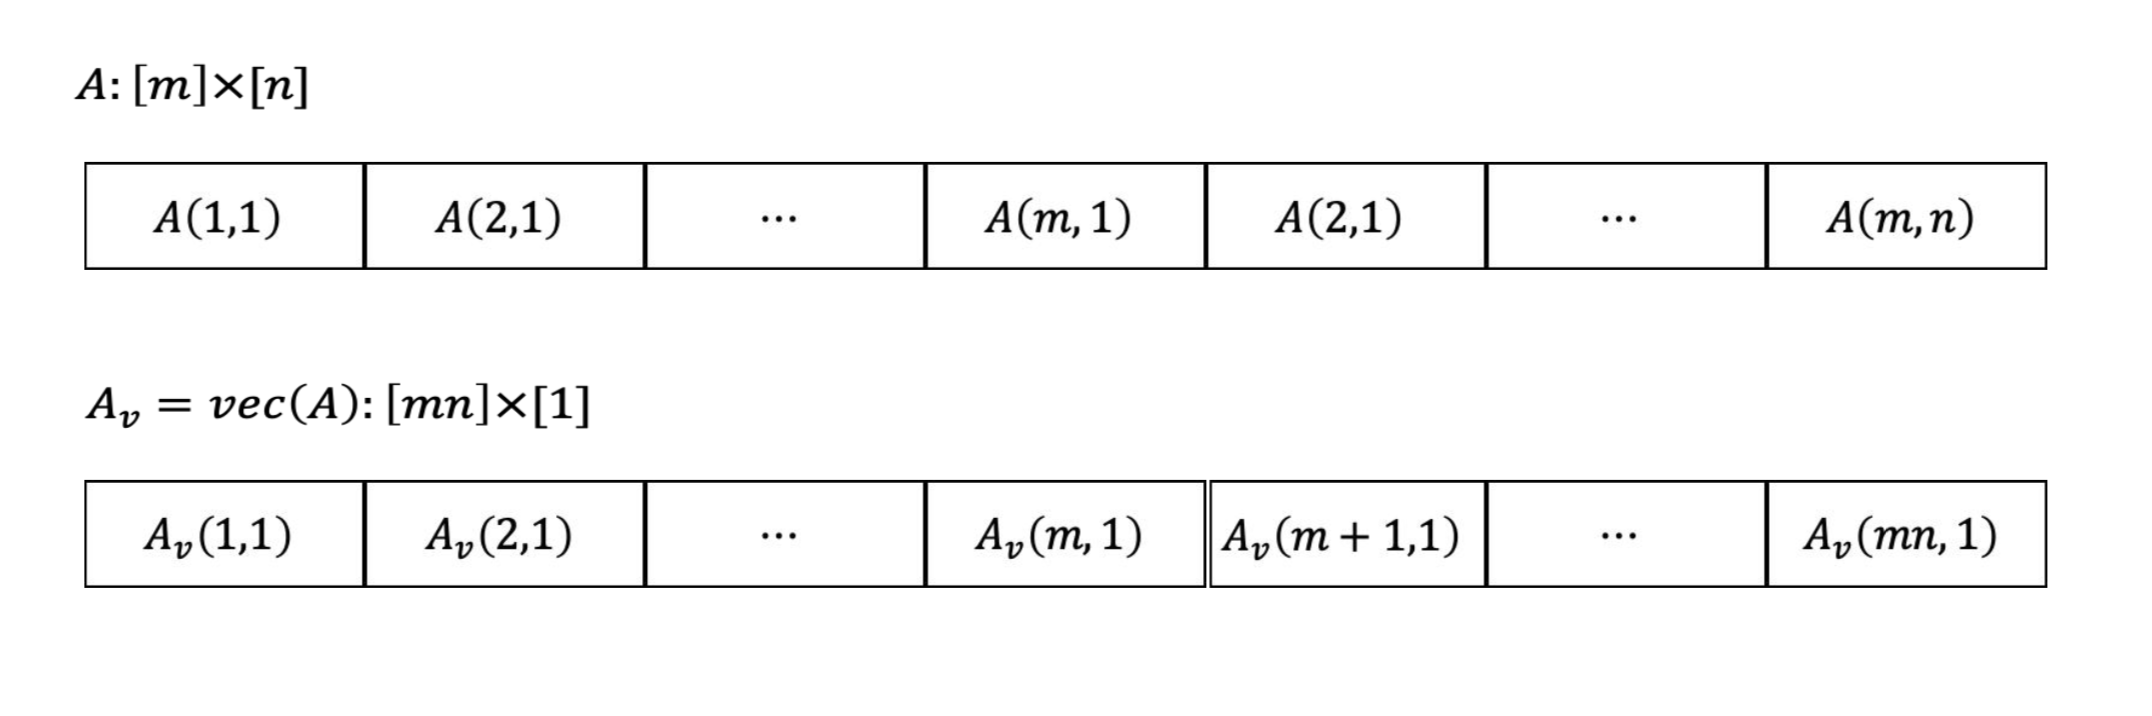
\includegraphics[width=0.7\textwidth]{vec2mat.png}
\caption{Vectorize a matrix $\mathbf{A}$ into vec($\mathbf{A}$) in memory}
\label{Fig:vec2mat}
\end{figure}

\subsubsection{Multiply of Block Diagonal Matrices}
Using the operational properties of the block matrix we get:
\begin{equation}
        [\mathbf{A}_1, \mathbf{A}_2, \cdots, \mathbf{A}_{N_2}]
        \begin{bmatrix}
            \mathbf{U}^c & & & \\
            & \mathbf{U}^c & & \\
            & & \ddots & \\
            & & & \mathbf{U}^c
        \end{bmatrix}
        =
        [\mathbf{A}_1\mathbf{U}^c, \mathbf{A}_2\mathbf{U}^c, \cdots, \mathbf{A}_{N_2}\mathbf{U}^c]
\label{step1}
\end{equation}
It shows that multiplication of block diagonal matrices can be transformed into a batch of small matrix multiplications. As we use column-first format to store $\mathbf{A}$, the batch of $\mathbf{A}_i$ are stored in constant stride. Let $p$ indicate the location of the first element of $\mathbf{A}_0$, then the location of the first element of $\mathbf{A}_i$ is $p+i\times N_1N_3$.  We utilize the gemmStridedBatchd() routine in NVIDIA cuBLAS Library to compute a batch of matrix multiplications simultaneously to achieve better performance.
\begin{figure}[H]
\centering
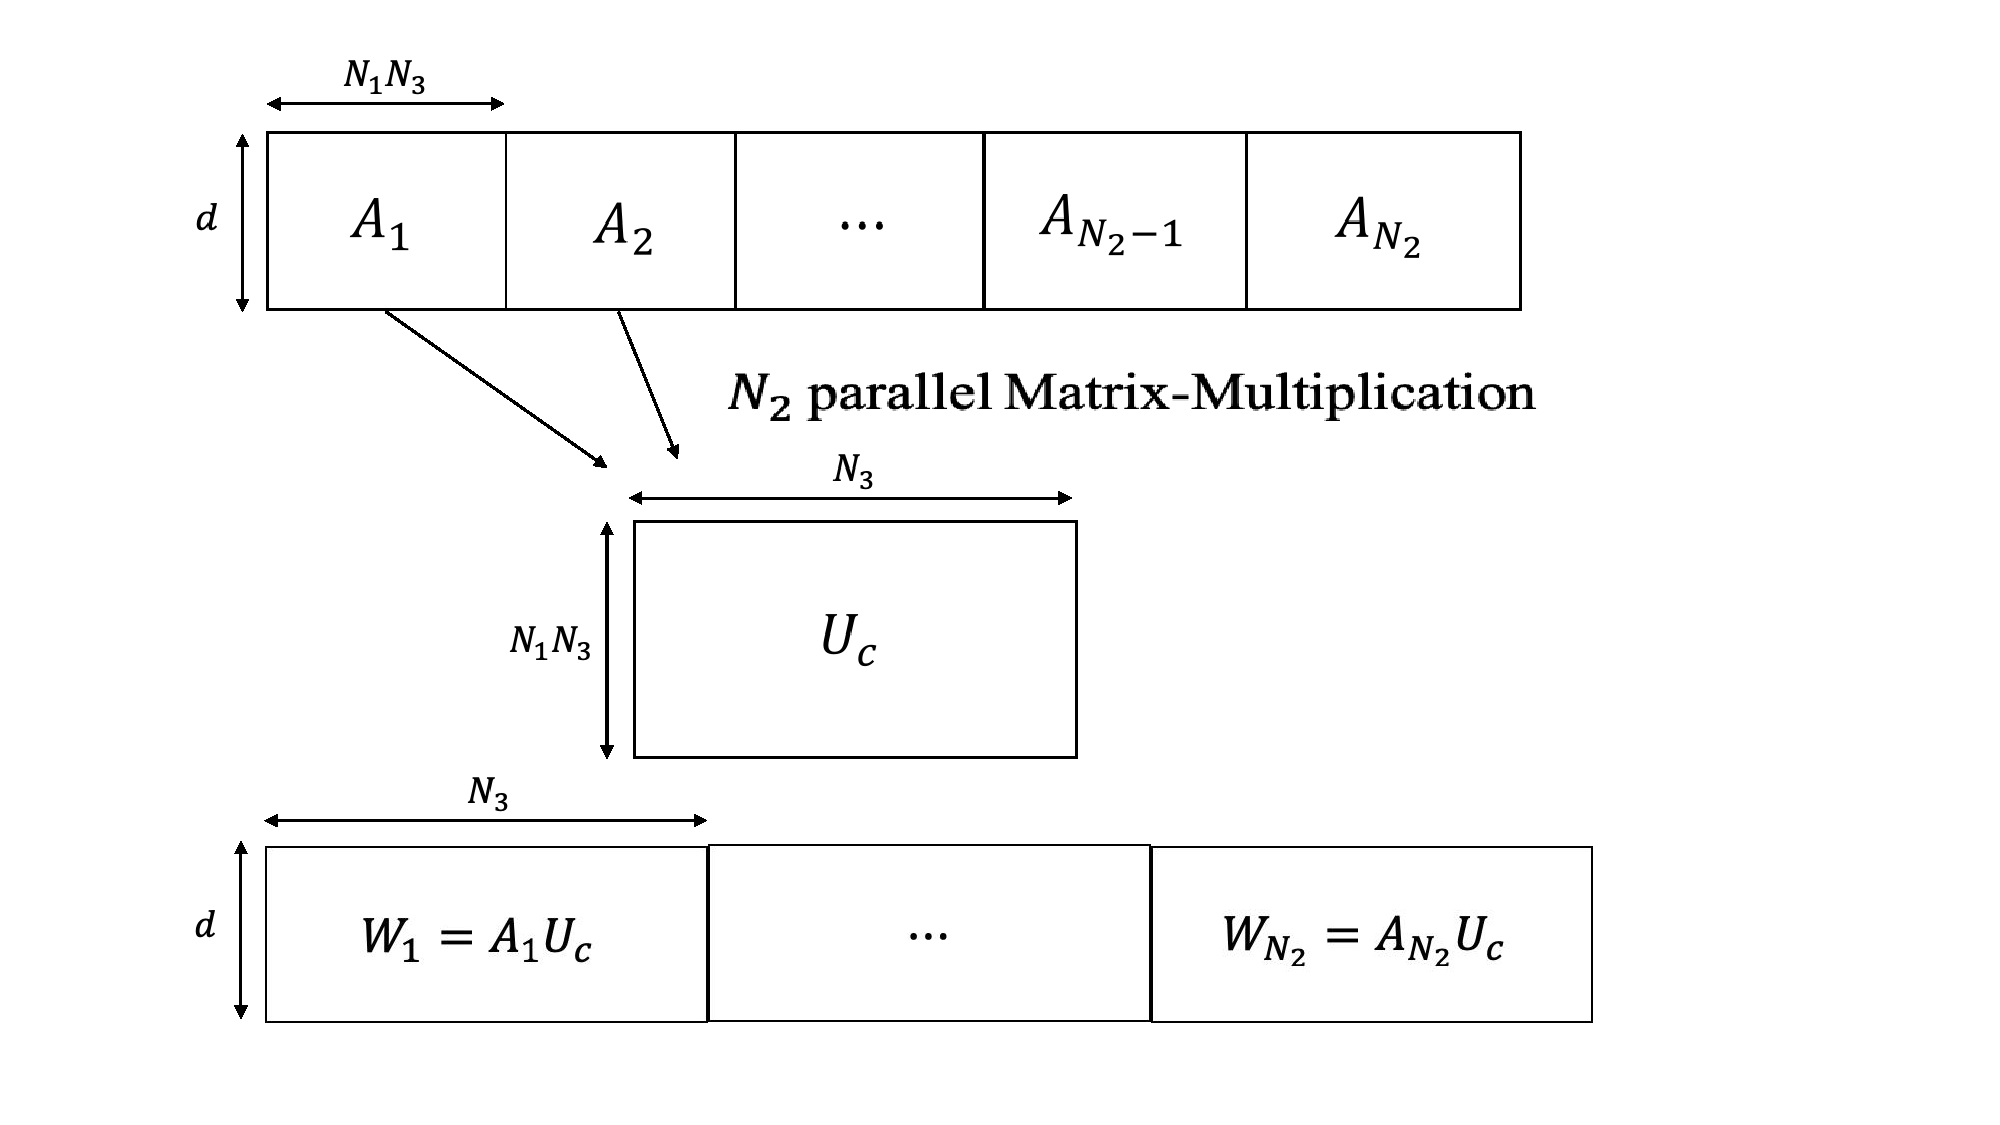
\includegraphics[width=0.7\textwidth]{diagMM.pdf}
\caption{Multiplication of block diagonal matrices on GPU}
\label{Fig:diagMM}
\end{figure}

\begin{table}
\caption{The parameters of the gemmStridedBatchd() routine in the cuBLAS library.}
\label{tab:gemm}
\begin{tabular}{|l|l|l|}
\hline
Parameters & Meaning & Value \\
\hline
transA & operation op($\mathbf{A}$) that is non- or transpose & non-transpose \\
\hline
transU & operation op($\mathbf{U}$) that is non- or transpose & transpose \\
\hline
$\mathbf{A}$ & pointer to the $\mathbf{A}$ matrix corresponding to the first instance of the batch & $d_A$ \\
\hline
$\mathbf{U}$ & pointer to the $\mathbf{U}$ matrix & $d_y$ \\
\hline
$\mathbf{W}$ & pointer to the $\mathbf{W}$ matrix & $d_W$ \\
\hline
strideA & the address offset between $\mathbf{A}_i$ and $\mathbf{A}_{i+1}$ & $M\times N_1N_3$ \\
\hline
strideU & the address offset between $\mathbf{U}_i$ and $\mathbf{U}_{i+1}$ & 0 \\
\hline
strideW & the address offset between $\mathbf{W}_i$ and $\mathbf{W}_{i+1}$ & $M\times N_3$ \\
\hline
batchNum & number of $gemm$ to perform in the batch & $N_2$ \\
\hline
\end{tabular}
\end{table}

\subsubsection{Eliminating Explicit Transpose Operations}
After each least squares method, the transpose of the target matrix is obtained. The transpose operation of the matrix needs to be performed (lines 6 and 12 in Alg. \ref{list:pseudocode}). However, the transpose operation takes a lot of computing time and resource. As the operation after transpose of the matrix is multiplication of diagonal matrices, we eliminate explicit matrix transpose by enabling the transpose option in the gemmStridedBatched() routine. In this way, the gemmStridedBatched() routine will perform matrix transpose implicitly and efficiently before the matrix multiplications. 

\subsubsection{Least Squares Minimization}
As shown in Alg. \ref{list:pseudocode}, least squares minimization (LSM) is the major step of the tensor sensing approach, which is the most time-consuming part of the entire approach. There are many approaches to perform least squares minimization. QR factorization is one of the most efficient approaches, which is well supported by CUDA.

\subsection{Optimizations of the GPU Tensor Sensing}
\label{SEC_OPT}
During the computation flow of the GPU tensor sensing, frequent data transfer between the CPU and GPU will significantly degrade system performance. Therefore we design data reusing  strategy to reduce data transfer overhead and resource consumption.

In the entire tensor sensing flow, we envoke data transfer only twice at the beginning and in the end. At the beginning, the input data is transferred from the CPU to the GPU. In the end, the final result matrix is sent back to the CPU. We optimize the computations in the tensor sensing flow such that they all perform in-place calculations. For instance, in the QR decomposition to solve the least squares problem, the input vector $\mathbf{y}$ is overrode by the result vectors (vec($\mathbf{U}$) and  vec($\mathbf{V}$)). Therefore, we need to reassign the vector $\mathbf{y}$ at the beginning of each least squares minimization iteration. However, it is an expensive operation to load the original data of vector $\mathbf{y}$ from the CPU memory every time. Instead, we pre-allocate a memory space named  $dyL$ on the GPU that stores the original data of the vector $\mathbf{y}$. Every time we need to reassign the $dy$, we use the GPU device to device transfer routine cudaMemcpyDeviceToDevice() to copy the data from $dyL$ to $dy$. Since the device to device bandwidth $~380 GB/s$ is much higher than the bandwidth between the CPU and GPU $~12 GB/s$, this strategy significantly reduces data transfer overhead. Alg.\ref{alg:GPU} and Fig.\ref{Fig:dataTS} describes the computation flow and data organization of the tensor sensing on the GPU.

%is that lsm using qr should be mentioned?
\begin{figure}[H]
\centering
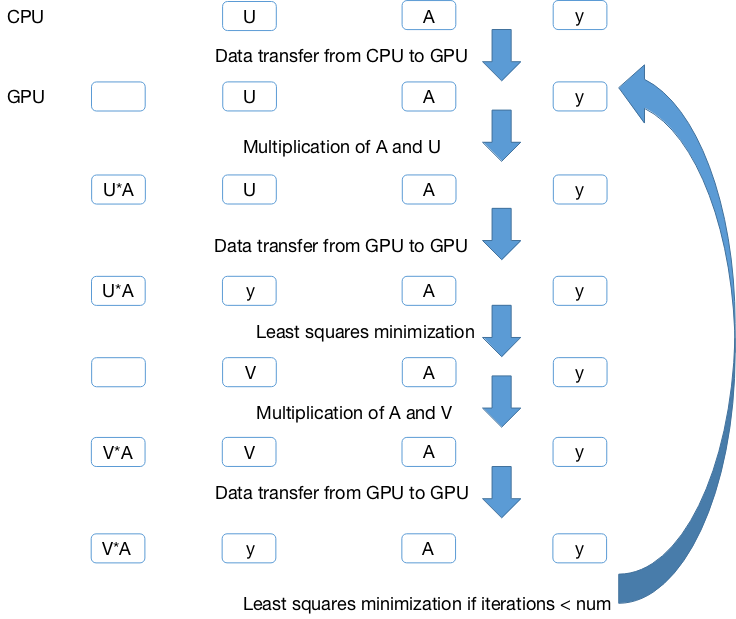
\includegraphics[width=0.7\textwidth]{dataTS.png}
\caption{Memory organization in the calculation process}
\label{Fig:dataTS}
\end{figure}

\begin{algorithm}
\setstretch{2}
\caption{Computation Flow of the Tensor Sensing on the GPU}
\label{alg:GPU}
\begin{algorithmic}[1]
    \Require Data on CPU memory: randomly initialized $\mathbf{U}^0$, measurement vector $\mathbf{y} \in \mathbf{R}^M$, matrix $\mathbf{A} \in \mathbb{R}^{M \times N_1N_2N_3}$ converted from $M$ sensing tensors $\mathcal{A}_m$
    \Ensure $\mathbf{X} \in \mathbb{R}^{N_1N_3 \times N_2}$
    \State apply for memory on GPU device: $dy, dA, dW, dyL$ ($dA(\mathcal{A})$ means that the content in $dA$ is $\mathcal{A}$, the same below)
    \State data transfer: $\mathcal{A}, \mathbf{y}, \mathbf{U}^0 \stackrel{cudaMemcpyHostToDevice}{\longrightarrow} dA(\mathcal{A}), dy(\mathbf{U}^0), dyL(\mathbf{y})$ 
    \For{$i=0 \to IterNum$}
        \State $dW(\text{uninitialized}), dA(\mathcal{A}), dy(\mathbf{U}^i) \stackrel{cublas<t>gemmStridedBatchd}{\longrightarrow} dW(\mathcal{A}\, \text{diag}(\mathbf{U}^i)), dA(\mathcal{A}), dy(\mathbf{U}^i)$
        \State  $dy(\mathbf{U}^i), dyL(\mathbf{y}) \stackrel{cudaMemcpyDeviceToDevice}{\longrightarrow} dy(\mathbf{y}), dyL(\mathbf{y})$
        \State $dW(\mathcal{A}\, \text{diag}(\mathbf{U}^i)), dy(\mathbf{y}) \stackrel{cusolver<t>qr}{\longrightarrow} dy(\mathbf{V}), dW(\text{uninitialized})$
        \State $dW(\text{uninitialized}, dA(\mathcal{A}), dy(\mathbf{V}^i))e \stackrel{cublas<t>gemmStridedBatchd}{\longrightarrow} dW(\mathcal{A}\, \text{diag}(\mathbf{V}^i)), dA(\mathcal{A}), dy(\mathbf{V}^i)$
        \State  $dy(\mathbf{V}^i), dyL(\mathbf{y}) \stackrel{cudaMemcpyDeviceToDevice}{\longrightarrow} dy(\mathbf{y}), dyL(\mathbf{y})$
        \State $dW(\mathcal{A}\, \text{diag}(\mathbf{V}^i)), dy(\mathbf{y}) \stackrel{cusolver<t>qr}{\longrightarrow} dy(\mathbf{U}^i), dW(\text{uninitialized})$
    \EndFor
    \State \Return $\mathbf{X} = \mathbf{U}\mathbf{V}$
\end{algorithmic}
\end{algorithm}

\section{Experiment Methodology}
\label{SEC_EXP}
In this section, we describe the experiment methodology including the hardware and software platform, testing data, testing process, and the comparison metrics.

\subsection{Hardware and Software Platform}
We use an NVIDIA Tesla V100 GPU to evaluate the performance of GPU tensor sensing. The GPU incorporates 5120 CUDA cores @ 1.53 GHz and 32 GB DDR5 memory. It is installed on a server with 128 GB DDR memory and an Intel i7-7820x CPU with 8 cores @ 3.60 GHz supporting 16 hardware threads with hyperthreading technology. The server is running Ubuntu 18.04 LTS with the kernel version 4.15.0. The CPU and GPU tensor sensing is running with Matlab R2017b and  CUDA 10.0, repectively.

\subsection{Testing Data}
In the experiment, we use both ground-truth and synthetic data in the evaluation. For ground-truth data, we use the IKEA 3D data (\ref{F Artificial data does not correspond to a specific physical model. We use this data to demonstrate the performance of our approach at different data sizes.ig:chair}) that generates a ground truth tensor of size $40 \times 40 \times 6$ with $\mathcal{L}$-rank 1. Each 3D model is placed in the middle of the “tensor” and occupies a part of the space. In this task, we mainly focus on the location and outline information, while the texture and color information are ignored. The synthetic data is generated according to the compressed sensing model \cite{matsuda2017multi}. The synthetic data does not correspond to a specific physical model. We use it to demonstrate the performance of our approach at different data sizes.
\begin{figure}[t]
\centering
\subfigure[]{
        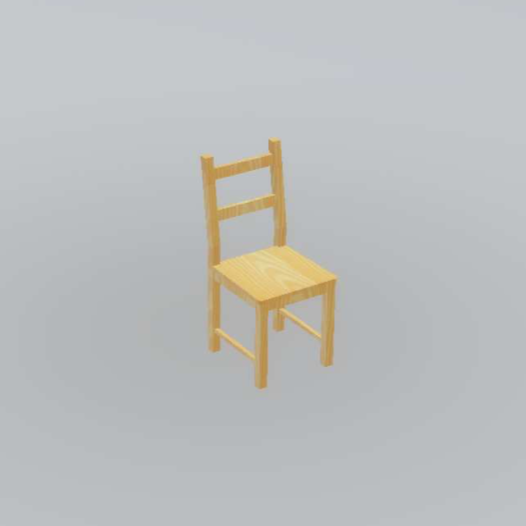
\includegraphics[width=0.4\textwidth]{chairOr.png}
    }
\subfigure[]{
        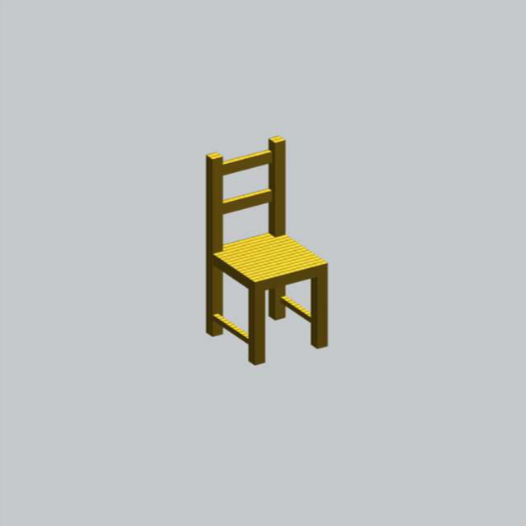
\includegraphics[width=0.4\textwidth]{chairRe.png}
    }
\caption{(a) is the 3D visualization of an IKEA models, (b) is the corresponding recovery results.}
\label{Fig:chair}
\end{figure}

\subsection{Testing Process}
The synthetic and real data are processed by the CPU tensor sensing implementation in Matlab and GPU tensor sensing implementation in CUDA, respectively. We evaluate and compare two versions of GPU tensor sensing: the unoptimized one and the optimized one. The unoptimized GPU tensor sensing adopts none of the optimization techniques in Sec. \ref{SEC_OPT}.  We repeat each experiment five times and report the average results.

\subsection{Comparison Metrics}
We adopt two metrics for comparison: running time and relative error rate.
\begin{itemize}
    \item \textit{Running time:} varying the tensor size and fixing other parameter, we measure the execution time of the CPU tensor sensing, unoptimized GPU tensor sensing and optimized GPU tensor sensing. Finally we calculate speedups as the running time of the CPU tensor sensing divided by the running time of GPU tensor sensing.
    \item \textit{error rate:} we adopt the metric relative square error, defined as $ RSE = \| \widehat{\mathcal{X}} - \mathcal{X} \|_F / \|\mathcal{X} \|_F $.
\end{itemize}

\section{Results and Analysis}
\label{SEC_RESULT}
\subsection{Running Time of Synthetic Data}
\begin{figure}[t]
    \centering
    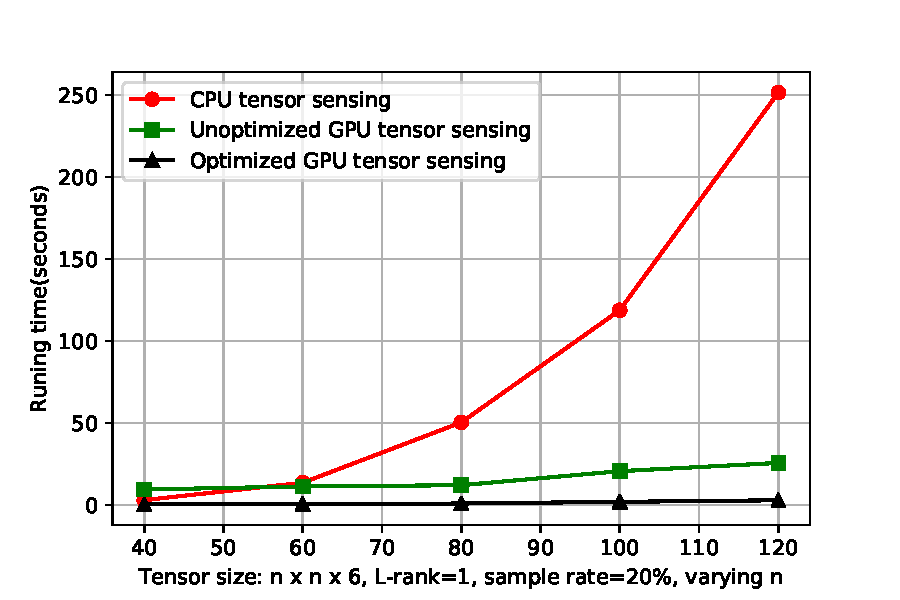
\includegraphics[width=3.5in]{runtime.pdf}
    \caption{Running time of the CPU tensor sensing and GPU tensor sensing}
    \label{pic:runtime}
\end{figure}

\begin{table}[t]
  \renewcommand{\arraystretch}{1.3}
  \centering
  \scriptsize
  \caption{Running time under varying tensor size ($n \times n \times 6$).}
  \begin{tabular}{|l|l|l|l|l|l|}
    \hline
    \textbf{\textbf{n}} & \textbf{40}& \textbf{60}& \textbf{80} & \textbf{100} & \textbf{120}\\
    \hline
    CPU tensor sensing time (S) & 3.07 & 13.65 & 50.43 & 118.84 & 251.54\\
    \hline
    Unoptimized GPU tensor sensing time (S) & 9.50 & 11.40 & 12.15 & 20.70 & 25.74\\
    \hline
    Optimized GPU tensor sensing time (S) & 0.44 & 0.63 & 0.98 & 2.01 & 2.97\\
    \hline
    Speedups-unoptimized & 0.32 & 1.20 & 4.15 & 5.74 & 9.77\\
    \hline
    Speedups-optimized & 6.98 & 21.67 & 51.46 & 59.12 & 84.70\\
    \hline
  \end{tabular}
  \label{tbl_runtime}
\end{table}

Fig. \ref{pic:runtime} shows that the running time of the CPU tensor sensing and two GPU tensor sensing implementations (unoptimized and optimized ones) for $\mathcal{X}$ of size $n\times n \times 6$ of $\mathcal{L}$-rank 1, where $n$ varies from 40 to 120 at a step of 20. The sampling rate is set to 20\%, and both CPU and GPU tensor sensing iterate 5 iterations for completion. The detailed time value is listed in Table \ref{tbl_runtime}. 
While $M = N_1 \times N_2 \times N_3 \times \text{sampling rate}$ and $\mathcal{A} \in \mathbb{R}^{M \times N_1N_2N_3}$, the scale of the main operation matrix $\mathcal{A}$ increases at a rate of four times as the increase rate of $n$. 

We can see that the running time of the CPU tensor sensing is polynomial with the increase of $n$, while the running time of the GPU tensor sensing is linearly growing. The unoptimzed and optimized GPU tensor sensing achieved an average of $4.24 \times$ and $44.79 \times$ and up to $9.77 \times$ and $84.70 \times$ speedups, respectively. This illustrates the effectiveness of the optimization methods proposed in Sec. \ref{SEC_OPT}. When the tensor size is small, the data transfer occupies a major portion of the entire execution time of the unoptimized GPU tensor sensing. As a result, its performance is even lower than the CPU tensor sensing.

\begin{figure}[t]
    \centering
    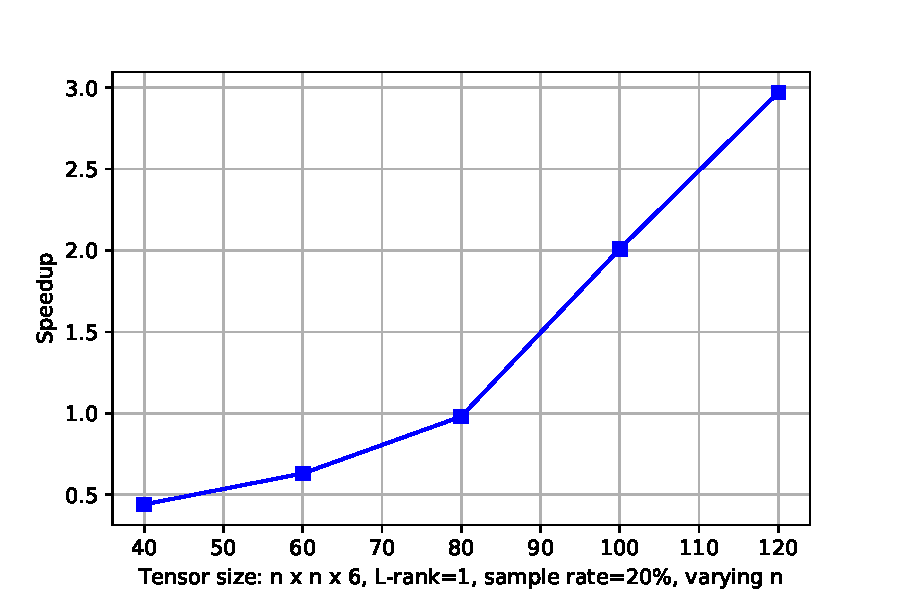
\includegraphics[width=3.5in]{speedup.pdf}
    \caption{Speedups of the unoptimized and optimized GPU tensor sensing.}
    \label{pic:runtime}
\end{figure}

\subsection{Error Rate and Running Time of Ground-truth Data}
\begin{figure}[t]
    \centering
    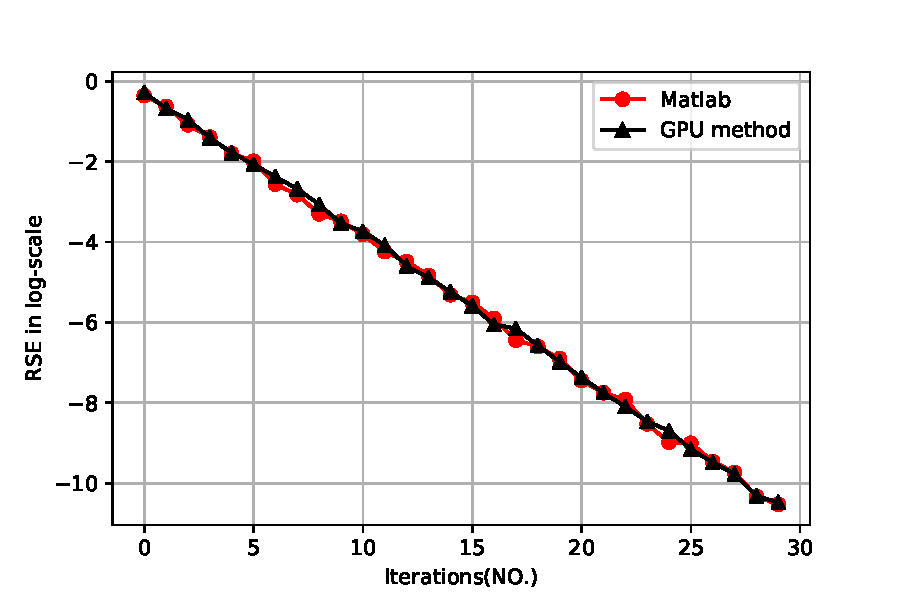
\includegraphics[width=3.5in]{rse.pdf}
    \caption{RSE of the CPU tensor sensing and GPU tensor sensing.}
    \label{pic:rse}
\end{figure}

This experiment evaluate the error rate of the CPU and GPU tensor sensing under different iterations for $\mathcal{X}$ of size $40 \times 40 \times 6$ with $\mathcal{L}$-rank 1. The sampling rate is set to 50\%. The running time of the CPU tensor sensing at 5 iterations is 14.91 seconds on average, while the running time of the GPU tensor sensing is 0.97 second on average, thus the speedup is $15.37 \times$. As shown in Fig. \ref{pic:rse}, under increased iterations from 1 to 30, the RSEs drop significantly. More importantly, the CPU tensor sensing and GPU implementation achieve almost the same RSEs at all iterations ( the two curves in Fig. \ref{pic:rse} overlap with each other), which means that they achieve similar error rate performance in tensor sensing.

\section{Conclusions}
\label{SEC_CON}
In this work, we present an open-source library named \textit{cuTensorSensing} for efficient RF tomographic imaging on GPUs. The experiment evaluations show that the proposed GPU tensor sensing works effectively and accurately. Compared with the counterpart on CPU, the GPU tensor sensing achieves similar error rate but much faster speed. For synthetic data, the GPU tensor sensing achieves an average of $44.79 \times$ and up to $84.70 \times$ speedups versus the CPU tensor sensing for bigger tensors. For ground-truth 3D objects data of smaller tensor size, the GPU tensor sensing achieves a $15.37 \times$ speedup over the CPU tensor sensing. The cuTensorSensing library is useful for efficient RF tomographic imaging.

%%%%%%%%%%%%%%%%%%%%%%%%%%%%%%%%%%%%%%%%%%
%\section{Patents}
%This section is not mandatory, but may be added if there are patents resulting from the work reported in this manuscript.

%%%%%%%%%%%%%%%%%%%%%%%%%%%%%%%%%%%%%%%%%%
\vspace{6pt} 

%%%%%%%%%%%%%%%%%%%%%%%%%%%%%%%%%%%%%%%%%%
%% optional
%\supplementary{The following are available online at \linksupplementary{s1}, Figure S1: title, Table S1: title, Video S1: title.}

% Only for the journal Methods and Protocols:
% If you wish to submit a video article, please do so with any other supplementary material.
% \supplementary{The following are available at \linksupplementary{s1}, Figure S1: title, Table S1: title, Video S1: title. A supporting video article is available at doi: link.}

%%%%%%%%%%%%%%%%%%%%%%%%%%%%%%%%%%%%%%%%%%
\authorcontributions{abstract, introduction, related works, conclusions and the revising of the entire manuscript, Tao Zhang; algorithms, experiments, and results, Da Xu.}


%%%%%%%%%%%%%%%%%%%%%%%%%%%%%%%%%%%%%%%%%%
\funding{This research is partially supported by Natural Science Foundation of Shanghai under grant No. 17ZR1409800, Science and technology committee of Shanghai Municipality under grant No. 16010500400.}

%%%%%%%%%%%%%%%%%%%%%%%%%%%%%%%%%%%%%%%%%%
\acknowledgments{The authors would like to thank anonymous reviewers for their fruitful feedback and comments that have helped them improve the quality of this work.}

%%%%%%%%%%%%%%%%%%%%%%%%%%%%%%%%%%%%%%%%%%
\conflictsofinterest{The authors declare no conflict of interest.} 

%%%%%%%%%%%%%%%%%%%%%%%%%%%%%%%%%%%%%%%%%%
%% optional
%\abbreviations{The following abbreviations are used in this manuscript:\\

%\noindent 
%\begin{tabular}{@{}ll}
%MDPI & Multidisciplinary Digital Publishing Institute\\
%DOAJ & Directory of open access journals\\
%TLA & Three letter acronym\\
%LD & linear dichroism
%\end{tabular}}

%%%%%%%%%%%%%%%%%%%%%%%%%%%%%%%%%%%%%%%%%%
%% optional
%\appendixtitles{no} %Leave argument "no" if all appendix headings stay EMPTY (then no dot is printed after "Appendix A"). If the appendix sections contain a heading then change the argument to "yes".
%\appendixsections{multiple} %Leave argument "multiple" if there are multiple sections. Then a counter is printed ("Appendix A"). If there is only one appendix section then change the argument to "one" and no counter is printed ("Appendix").
%\appendix
%\section{}
%\unskip
%\subsection{}
%The appendix is an optional section that can contain details and data supplemental to the main text. For example, explanations of experimental details that would disrupt the flow of the main text, but nonetheless remain crucial to understanding and reproducing the research shown; figures of replicates for experiments of which representative data is shown in the main text can be added here if brief, or as Supplementary data. Mathematical proofs of results not central to the paper can be added as an appendix.

%\section{}
%All appendix sections must be cited in the main text. In the appendixes, Figures, Tables, etc. should be labeled starting with `A', e.g., Figure A1, Figure A2, etc. 

%%%%%%%%%%%%%%%%%%%%%%%%%%%%%%%%%%%%%%%%%%
% Citations and References in Supplementary files are permitted provided that they also appear in the reference list here. 

%=====================================
% References, variant A: internal bibliography
%=====================================
\reftitle{References}
%\begin{thebibliography}{999}
% Reference 1
%\bibitem[Author1(year)]{ref-journal}
%Author1, T. The title of the cited article. {\em Journal Abbreviation} {\bf 2008}, {\em 10}, 142-149, doi:xxxxx.
% Reference 2
%\bibitem[Author2(year)]{ref-book}
%Author2, L. The title of the cited contribution. In {\em The Book Title}; Editor1, F., Editor2, A., Eds.; Publishing House: City, Country, 2007; pp. 32-58, ISBN.
%\end{thebibliography}

% The following MDPI journals use author-date citation: Arts, Econometrics, Economies, Genealogy, Humanities, IJFS, JRFM, Laws, Religions, Risks, Social Sciences. For those journals, please follow the formatting guidelines on http://www.mdpi.com/authors/references
% To cite two works by the same author: \citeauthor{ref-journal-1a} (\citeyear{ref-journal-1a}, \citeyear{ref-journal-1b}). This produces: Whittaker (1967, 1975)
% To cite two works by the same author with specific pages: \citeauthor{ref-journal-3a} (\citeyear{ref-journal-3a}, p. 328; \citeyear{ref-journal-3b}, p.475). This produces: Wong (1999, p. 328; 2000, p. 475)

%=====================================
% References, variant B: external bibliography
%=====================================
\externalbibliography{yes}
\bibliography{mybibfile}

%%%%%%%%%%%%%%%%%%%%%%%%%%%%%%%%%%%%%%%%%%
%% optional

%% for journal Sci
%\reviewreports{\\
%Reviewer 1 comments and authors’ response\\
%Reviewer 2 comments and authors’ response\\
%Reviewer 3 comments and authors’ response
%}

%%%%%%%%%%%%%%%%%%%%%%%%%%%%%%%%%%%%%%%%%%
\end{document}
